%%%%%%%%%%%%%%%%%%%%%%%%%%%%%%%%%%%%%%%%%%%%%%%%%%%
%% P3: Phenomenology of Particle Physics                         
%%
%% Author:  André Rubbia                   		 
%%
%% Figure 4.5 The integration in the Dyson series.
%%
%% This work is licensed under the Creative Commons Attribution 4.0 International License. 
%% To view a copy of this license, visit http://creativecommons.org/licenses/by/4.0/ or 
%% send a letter to Creative Commons, PO Box 1866, Mountain View, CA 94042, USA.
%%
%%%%%%%%%%%%%%%%%%%%%%%%%%%%%%%%%%%%%%%%%%%%%%%%%%%

\documentclass[a4paper,10pt]{article}

\usepackage[T1]{fontenc}
\usepackage[utf8]{inputenc}
\usepackage{lmodern}
\usepackage[labelfont=bf]{caption}
\usepackage{upgreek}

\usepackage{tikz}
\usepackage{pgfplots}
\pgfplotsset{compat=1.17}
\usepgfplotslibrary{ternary}
\usepgfplotslibrary{fillbetween}
\usepgfplotslibrary{external}

\def\d{\mathrm{d}}

\begin{document}

%%%%%%%%%%%%%%%   FIGURE  %%%%%%%%%%%%%%%%%%%%%%%%%%%%%%
\begin{figure}[htb]
\begin{center}
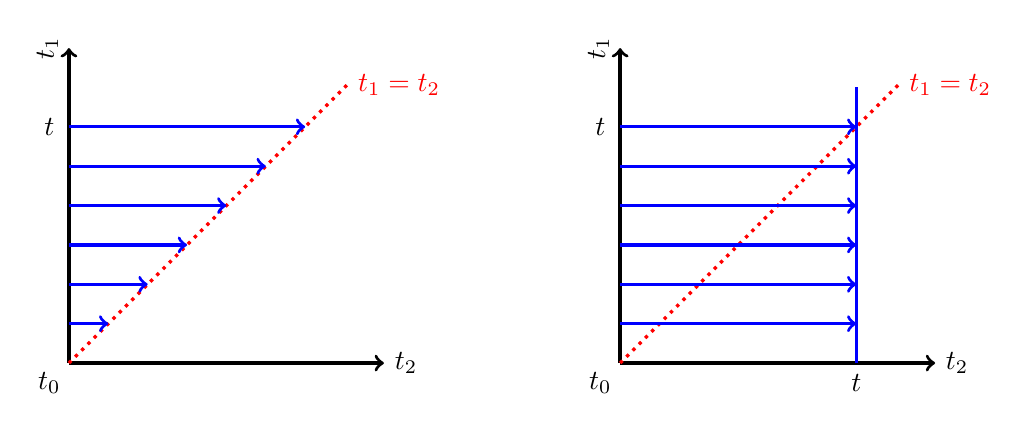
\begin{tikzpicture}[scale=1.0]
\begin{scope}[shift={(0,0)}]
\draw[black,very thick,->] (0,0) -- +(90:4) node[above,rotate=90] {$t_1$};
\draw[black,very thick,->] (0,0) -- +(0:4) node[right] {$t_2$};
\draw[red,very thick,dotted] (0,0) -- +(45:5) node[right] {$t_1=t_2$};
\draw[blue,very thick,->] (0,1) -- +(0:1);
\draw[blue,very thick,->] (0,2) -- +(0:2);
\draw[blue,very thick,->] (0,3) -- +(0:3);
\draw[blue,very thick,->] (0,0.5) -- +(0:0.5);
\draw[blue,very thick,->] (0,1.5) -- +(0:1.5);
\draw[blue,very thick,->] (0,2.5) -- +(0:2.5);
\node at (-0.25,3) {$t$};
\node at (-0.25,-0.25) {$t_0$};
\end{scope}
\begin{scope}[shift={(7,0)}]
\draw[black,very thick,->] (0,0) -- +(90:4) node[above,rotate=90] {$t_1$};
\draw[black,very thick,->] (0,0) -- +(0:4) node[right] {$t_2$};
\draw[red,very thick,dotted] (0,0) -- +(45:5) node[right] {$t_1=t_2$};
\draw[blue,very thick,->] (0,1) -- +(0:3);
\draw[blue,very thick,->] (0,2) -- +(0:3);
\draw[blue,very thick,->] (0,3) -- +(0:3);
\draw[blue,very thick,->] (0,0.5) -- +(0:3);
\draw[blue,very thick,->] (0,1.5) -- +(0:3);
\draw[blue,very thick,->] (0,2.5) -- +(0:3);
\draw[blue,very thick] (3,0) -- +(90:3.5);
\node at (-0.25,3) {$t$};
\node at (3,-0.25) {$t$};
\node at (-0.25,-0.25) {$t_0$};
\end{scope}
\end{tikzpicture}
\caption{(left) The integration in the Dyson series with $t_0<t_2<t_1<t$;
(right) the time-ordered integral with $t_0<t_1<t$ and $t_0<t_2<t$.}
\end{center}
\end{figure}
%%%%%%%%%%%%%%%   END FIGURE  %%%%%%%%%%%%%%%%%%%%%%%%%%%%%%
%

\end{document}
